\subsection{Spettro delle sorgenti a disposizione}

La nostra sorgente di \na{} ha 3 modi di decadimento:
\begin{itemize}
\item decadimento $\beta^+$ con $E_e=\SI{545}{keV}$, BR=90.4\%;
\item cattura elettronica (BR=9.5\% ) con la conseguente emissione di un fotone di energia \SI{1274}{keV} da parte del $^{22}$Ne formatosi;
\item decadimento $\beta^-$ con BR=0.1\%.
\end{itemize}

Useremo i decadimenti $\gamma$ del \cs{} (\SI{662}{keV}) e del \co{} (\SI{1173}{keV}, \SI{1332}{keV}) per calibrare il nostro apparato.

\marginpar{Scrivere perché non usiamo l'americio?}

\subsection{Fenomenologia dei rivelatori}

\marginpar{Scrivere materiale e dimensioni nella sezione ``apparato''}

Nel range di energie dei fotoni in cui lavoriamo, i processi di diffusione possibili sono gli scattering Rayleigh e Compton e l'effetto fotoelettrico.
Lo scattering Rayleigh, in quanto completamente elastico, non rilascia energia nel calorimetro.
Nella diffusione Compton il fotone cede una parte dell'energia ad un elettrone del nostro calorimetro e possiamo misurare l'energia persa da quest'ultimo. L'energia persa dal fotone segue la distribuzione di Klein-Nishina.
\marginpar{Klein-Nishina è la distribuzione angolare, non dell'energia.}
Se il fotone esegue un effetto fotoelettrico, perde tutta la sua energia cedendola ad un elettrone ed è l'unico modo che abbiamo per conoscere l'energia del fotone incidente.

A questo quadro si possono aggiungere processi di ordine superiore, come un numero maggiore di rimbalzi Compton all'interno del cristallo oppure un effetto fotoelettrico eseguito dopo uno scattering Compton.
Vedremo in seguito che un fotone, dopo aver eseguito un Compton all'interno di un rivelatore, può uscirne ed essere rivelato anche da un altro.

Riportiamo in \autoref{sezioni} un grafico che rappresenta la sezione d'urto dell'effetto Compton confrontata con quella del fotoelettrico all'interno del NaI. Per energie minori di \SI{200}{keV} l'effetto fotoelettrico domina sul Compton e viceversa per energie maggiori.
\marginpar{Dal grafico mi sembra più \SI{300}{keV}.}
Trascuriamo la produzione di coppie perché, quando è sopra soglia ($E_{\gamma}>\SI{1}{MeV}$), è 5 volte più piccola della sezione d'urto del fotoelettrico che, in questo range, è molto soppressa rispetto al Compton.
\marginpar{La caption di \autoref{fig:cross} è poco chiara, $\lambda$ è quello del grafico ma non c'è scritto da nessuna parte.}

\begin{figure}[h]
\centering
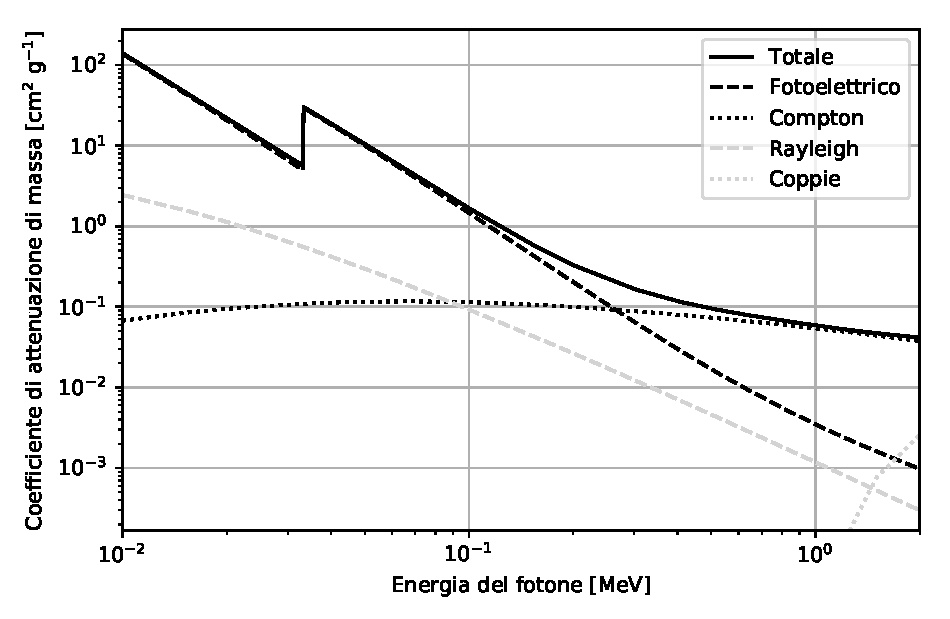
\includegraphics[width=25 em]{immagini/cross}
\caption{\label{fig:cross}
Sezioni d'urto in funzione dell'energia all'interno del nostro cristallo di NaI ($\rho=\SI{3.67}{g\,cm^{-3}})$ espressa come $\sigma=\frac{1}{\rho\lambda}$. Queste informazioni sono tratte da \cite{cross}.}
\label{sezioni}
\end{figure}
